\documentclass{article}
\usepackage{mainPoly}

\title{Expériences aléatoires et Probabilités}
\author{Seconde 9}
\date{}

\begin{document}
\maketitle
\section{Vocabulaire des probabilités}
\subsection{Univers}
\begin{definitionbox}
Une \emph{expérience aléatoire} est une expérience\dots
\begin{itemize}
\item dont les résultats \emph{possibles} sont connus;
\item mais dont le résultat \emph{obtenu} n'est pas prévisible.
\end{itemize}
\end{definitionbox}
\begin{example} Les exemples suivants sont des expériences aléatoires :
\begin{enumerate}
\item On lance un dé équilibré à six faces, et on regarde le nombre obtenu.
\label{dice}
\item On tire une carte dans un jeu de 52 cartes, et on regarde la couleur (♡,♢,♠,♣) obtenue. 
\label{cards}
\end{enumerate}
\end{example}
\begin{definitionbox}
\begin{itemize}
\item L'un des résultats possible d'une expérience aléatoire est appelé \emph{issue}.
\item L'\emph{univers} d'une expérience aléatoire est l'ensemble de ses issues.
\end{itemize}
\end{definitionbox}
\begin{example}
Pour définir l'univers d'une expérience aléatoire, on met entre accolades toutes ses issues. On appelle cet univers $\Omega$ qui se lit \og Oméga \fg.
\begin{enumerate}
\item L'univers de l'experience \ref{dice} est $\Omega = \{1;2;3;4;5;6\}$ 
\item L'univers de l'experience \ref{cards} est $\Omega = \{♡;♢;♠;♣\}$ 
\end{enumerate}    
\end{example}
\begin{exercize}
Donner l'univers des expériences aléatoire suivantes.
\begin{enumerate}[label=\alph*)]
\item On demande à un ou une élève du lycée s'il préfère les chats ou les chiens.
\item Un ou une camarade de classe choisit un nombre pair entre $1$ et $11$.
\item On lance deux dés équilibrés et on regarde la somme des résultats obtenus.
\end{enumerate}
\end{exercize}
\emptybox{7cm}
\newpage
\subsection{\'Evénements}
\begin{definitionbox}
Un \emph{événement} d'une expérience aléatoire est un ensemble contenant tout ou partie des issues de l'expérience aléatoire.
\end{definitionbox}
\begin{example}
\begin{enumerate}
\item Soit $A = \{1;3;5\}$. C'est un événement de l'expérience \ref{dice} (lancer de dé) : il correspond à \og Obtenir un impair \fg.
\item Soit $B = \{♠;♣\}$. C'est un événement de l'expérience \ref{cards} (tirage d'une carte) : il correspond à \og La carte tirée est noire \fg.
\end{enumerate}
\end{example}
\begin{vocabulary}
\begin{itemize}
\item Un événement \emph{certain} est un événement qui contient toutes les issues de l'expérience.  
\item Un événement \emph{impossible} est un événement qui ne contient aucun élément. On le note $\emptyset$.
\end{itemize}
\end{vocabulary}
\begin{exercize}
Compléter le tableau suivant :
\begin{center}
\begin{tabular}{|C{0.25\textwidth}|C{0.3\textwidth}|C{0.2\textwidth}|C{0.2\textwidth}|}
\hline
Expérience aléatoire & Univers $\Omega$ & \'Evénement $A$ & Issues de $A$ \\
\hline
On lance un dé équilibré à $6$ faces et on observe le résultat. & $\{1;2;3;4;5;6\}$ & Le nombre obtenu est pair. & $\{2;4;6\}$ \\
\hline
On lance une pièce équilibrée. & $\{\text{Pile};\text{Face}\}$ & On tombe sur Pile. & \\
\hline
On choisit un animal au hasard dans un zoo. & $\{\text{Lion};\text{Singe};\text{Perroquet}\}$ & L'animal choisi a des plumes. & \\
\hline
On choisit un jour de la semaine au hasard. & & On a sélectionné un jour du week-end. & $\{\text{Samedi};\text{Dimanche}\}$\\
\hline
On lance deux dé équilibrés, et on soustrait le plus grand résultat par le plus petit. & & La différence obtenue est $6$. & \\
\hline
On lance deux pièces équilibrées. & $\{(P,P);(F,F),(P,F),(F,P)\}$ & Les deux pièces sont sur le même côté. & \\
\hline 
\end{tabular}
\end{center}
\end{exercize}
\newpage
\section{Combinaison d'événements}
Soit une expérience aléatoire d'univers $\Omega$, et deux événements $A$ et $B$.
\begin{definitionbox}
\begin{itemize}
\item La \emph{réunion} de $A$ et de $B$, notée $A \cup B$, est l'événement contenant toutes les issues de $A$ ainsi que celles de $B$.
\item L'\emph{intersection} de $A$ et $B$, notée $A \cap B$, est l'événement contenant les issues présentes à la fois dans $A$ et dans $B$ 
\end{itemize} 
\end{definitionbox}
\begin{center}
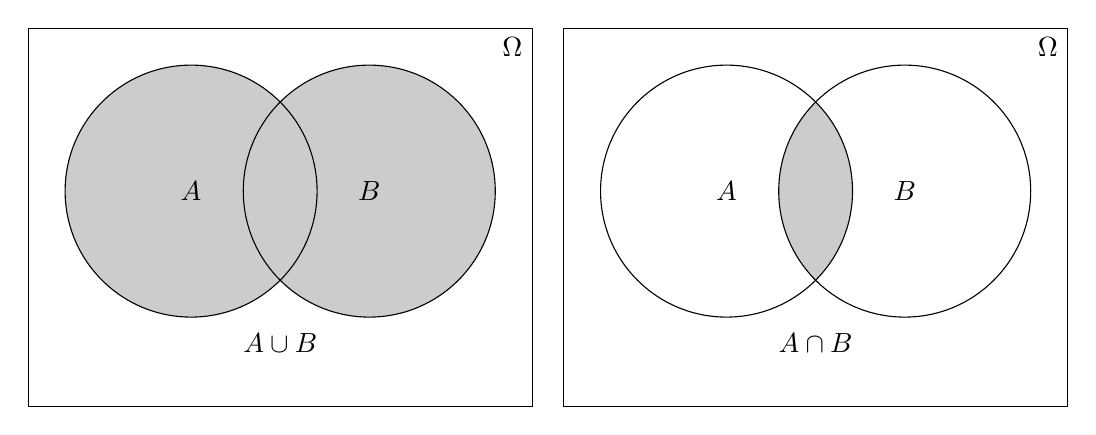
\begin{tikzpicture}[scale = 0.8]
\draw (-4,-2) rectangle (4,4) node[below left] {$\Omega$};
\begin{scope}
\clip (135:2) circle (2);
\fill[color=gray!40] (45:2) circle (2);
\end{scope}
\draw (135:2) node{$A$} circle (2);
\draw (45:2) node{$B$} circle (2);
\draw (0,-1) node{$A \cap B$};
\begin{scope}[xshift=-8.5cm]
\draw (-4,-2) rectangle (4,4) node[below left] {$\Omega$};
\fill[color=gray!40] (135:2) circle (2);
\fill[color=gray!40] (45:2) circle (2);
\draw (135:2) node{$A$} circle (2);
\draw (45:2) node{$B$} circle (2);
\draw (0,-1) node{$A \cup B$};
\end{scope}
\end{tikzpicture}
\end{center}
\begin{definitionbox}
Le \emph{complémentaire} de $A$, noté $\overbar{A}$, est l'ensemble des élément de $\Omega$ qui ne sont pas des éléments de $A$.
\end{definitionbox}
\begin{center}
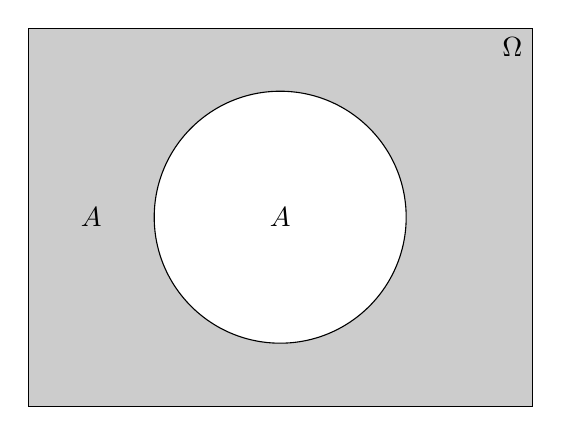
\begin{tikzpicture}[scale=0.8]
\fill[color=gray!40] (-4,-2) rectangle (4,4);
\draw (-4,-2) rectangle (4,4) node[below left] {$\Omega$};
\fill[color=white] (0,1) circle (2);
\draw (0,1) circle (2) node {$A$};
\draw (-3,1) node {$\overbar{A}$};
\end{tikzpicture}   
\end{center}
\vspace*{1cm}
\begin{example}
On lance un dé à 6 faces et on observe le résultat. Compléter le tableau ci-après.
\begin{center}
\begin{tabular}{|*{5}{C{0.15\textwidth}|}}
\hline
$A$ & $B$ & $A \cup B$ & $A \cap B$ & $\overbar{A}$\\
\hline
On obtient un nombre pair & On obtient un nombre supérieur ou égal à $4$ & $\{2;4;5;6\}$ & $\{4;6\}$ & $\{1;3;5\}$\\
\hline
On obtient un multiple de $3$ & On obtient un nombre inférieur à $2$ & & & \\
\hline
On obtient un $4$ & On obtient un $3$ & & & \\
\hline
\end{tabular}
\end{center}
\end{example}
\vspace*{1cm}
\begin{remark}
\begin{itemize}
\item En français, $A \cup B$ représente \og l'événement $A$ OU l'événement $B$ s'est réalisé.\fg
\item En français, $A \cap B$ représente \og l'événement $A$ ET l'événement $B$ se sont réalisés.\fg
\item En français, $\overbar{A}$ représente \og l'événement $A$ ne s'est pas réalisé.\fg
\end{itemize}
\end{remark}
\newpage
\section{Probabilités sur un univers fini}
\subsection{Loi de probabilité}
\begin{definitionbox}
Soit une expérience aléatoire dont l'univers est \emph{fini} : il est de la forme
\begin{equation*}
\Omega = \left\{e_1; e_2; \dots; e_n \right\}, \text{ avec } n \geq 1.
\end{equation*}

Une \emph{loi de probabilité} sur $\Omega$ est l'association de chaque issue $e_i$ à un nombre $p_i$ compris entre $0$ et $1$ inclus. De plus, la somme de tous ces nombres doit être égale à $1$.
\end{definitionbox}
\begin{example}
On lance un dé équilibré et on observe le résultat. Les deux associations ci-dessous sont des lois de probabilité.

\begin{center}
\begin{tabular}{|c|C{1cm}|C{1cm}|C{1cm}|C{1cm}|C{1cm}|C{1cm}|}
\hline
\Omega & $1$ & $2$ & $3$ & $4$ & $5$ & $6$\\
\hline\rule[-0.5cm]{0cm}{1cm}
Probabilités & $0$ & $0$ & $0$ & $0$ & $\dfrac{1}{2}$ & $\dfrac{1}{2}$\\
\hline
\end{tabular}
\end{center}
car $0 + 0 + 0 + 0 + \dfrac{1}{2} + \dfrac{1}{2} = 1$.
\begin{center}
\begin{tabular}{|c|C{1cm}|C{1cm}|C{1cm}|C{1cm}|C{1cm}|C{1cm}|}
\hline
\Omega & $1$ & $2$ & $3$ & $4$ & $5$ & $6$\\
\hline\rule[-0.5cm]{0cm}{1cm}
Probabilité & $\dfrac{1}{6}$ & $\dfrac{1}{6}$ & $\dfrac{1}{6}$ & $\dfrac{1}{6}$ & $\dfrac{1}{6}$ & $\dfrac{1}{6}$\\
\hline
\end{tabular}
\end{center}
car $\dfrac{1}{6} + \dfrac{1}{6} + \dfrac{1}{6} + \dfrac{1}{6} + \dfrac{1}{6} + \dfrac{1}{6} = 1$.
\end{example}
\begin{exercize}
Compléter le tableau suivant afin de définir une loi de probabilité sur $\Omega$. Cette loi de probabilité devra avantager les nombres impairs.
\begin{center}
\begin{tabular}{|c|*{6}{C{1cm}|}}
\hline
\Omega & $1$ & $2$ & $3$ & $4$ & $5$ & $6$\\
\hline\rule[-0.5cm]{0cm}{1cm}
Probabilité & & & & & & \\
\hline
\end{tabular}
\end{center}    
\end{exercize}
\begin{definition}
On dit qu'une expérience aléatoire est en \emph{situation d'équiprobabilité} si toutes les issues ont la même probabilité.
\end{definition}
\begin{example}
Les expériences aléatoires suivantes sont en situation d'équiprobabilité :
\begin{itemize}
\item Le lancer d'un dé équilibré.
\item Le lancer d'une pièce équilibrée.
\item Le tirage d'une carte dans un jeu de $52$ cartes mélangé.
\item Le tirage d'un jeton parmi des jetons indiscernables au toucher dans une urne opaque.  
\end{itemize}
\end{example}
\begin{definitionbox}
Soit $A$ un événement. La probabilité de $A$, notée $P(A)$, est la somme des probabilités des issues contenues par $A$.
\end{definitionbox}
\begin{example}
Pour la loi de probabilité donnée par l'exercice précédent, quelle est la probabilité de l'événement $A$\og Obtenir un nombre pair\fg ?
\end{example}
\emptybox{3cm}
\begin{remark}
\begin{equation*}
\begin{aligned}
P(\emptyset) &= 0\\
P(\Omega) &= 1 
\end{aligned}
\end{equation*}
\end{remark}
\newpage
\subsection{Calcul de Probabilités en situation d'équiprobabilité}
\begin{proposition}
Dans une expérience aléatoire d'univers $\Omega$ en situation d'équiprobabilité, la probabilité de $A$ est donnée par
\begin{equation*}
P(A)=\dfrac{\text{Nombre d'issues dans } A}{\text{Nombre d'issues dans }\Omega}
\end{equation*}
\end{proposition}
\begin{example}
\begin{enumerate}[label=\emph{\alph*)}]
\item On lance un dé équilibré. Quelle est la probabilité d'obtenir un multiple de $3$ ?
\item On lance deux dé équilibrés, un rouge et un bleu. Quelle est la probabilité que le dé rouge soit pair, et le dé bleu impair ?
\item On met dans un sac trois boules rouges, une boule bleue et une boule verte. Quelle est la probabilité de tirer une boule rouge ?
\item On tire une carte au hasard dans un jeu de $52$ cartes mélangé. Quelle est la probabilité de tirer une \og tête \fg (Valet, Dame, Roi) ?
\end{enumerate}
\end{example}
\emptybox{4cm}
\begin{tcolorbox}
Dans une situation d'équiprobabilité, il faut donc énumérer les cas favorables, puis diviser par le nombre de cas au total.
\end{tcolorbox}
\vspace*{1cm}

\begin{minipage}{0.45\textwidth}
\begin{example}
On tire au sort une personne dans un lycée de $1000$ personnes. Sachant qu'il y a $242$ secondes, $534$ premières, $632$ filles dont $320$ en terminale et $76$ en première, compléter le tableau suivant et donner la probabilité de tomber sur un garçon en seconde.
\begin{center}
\begin{tabular}{|c|c|c|c|c|}
\hline
            &Secondes   &Premières  &Terminale  &Total\\
\hline
Filles      &           &$76$       &$320$      &$632$\\
\hline
Garçons     &           &           &           &\\
\hline
Total       &$242$      &$534$      &           &$1000$\\
\hline
\end{tabular}
\end{center}
\emptybox{3cm} 
\end{example}
\end{minipage}
\hfill\vline\hfill
\begin{minipage}{0.45\textwidth}
\begin{example}
Dans un sac opaque contenant trois pièces d'or ($O_1$, $O_2$ et $O_3$) et une pièce d'argent ($A_1$), on tire deux pièces successivement et avec remise. En repassant sur les branches favorables, calculer la probabilité d'obtenir deux pièces d'or suite aux deux tirages.
\begin{center}
    
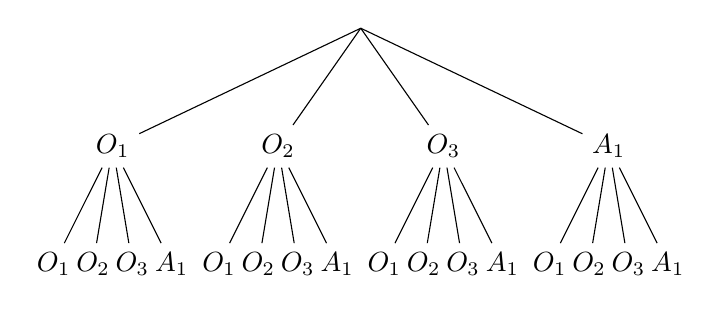
\begin{tikzpicture}
[
    level 1/.style={sibling distance=21mm},
    level 2/.style={sibling distance=5mm}]
\coordinate
    child {node {$O_1$}
        child {node {$O_1$}}
        child {node {$O_2$}}
        child {node {$O_3$}}
        child {node {$A_1$}}    
    }
    child {node {$O_2$}
        child {node {$O_1$}}
        child {node {$O_2$}}
        child {node {$O_3$}}
        child {node {$A_1$}}    
    }
    child {node {$O_3$}
        child {node {$O_1$}}
        child {node {$O_2$}}
        child {node {$O_3$}}
        child {node {$A_1$}}    
    }
    child {node {$A_1$}
        child {node {$O_1$}}
        child {node {$O_2$}}
        child {node {$O_3$}}
        child {node {$A_1$}}    
    }
;
\end{tikzpicture}
\end{center}
\emptybox{3cm}
\end{example}
\end{minipage}
\newpage
\subsection{Calcul de probabilités de combinaisons d'événements}
\begin{tcolorbox}
\begin{proposition}
Soit une expérience aléatoire d'univers fini $\Omega$, et deux événements $A$ et $B$. Alors,
\begin{equation*}
P(A \cup B) = P(A) + P(B) - P(A \cap B)
\end{equation*}
\end{proposition}
\end{tcolorbox}
\begin{remark}
La figure suivante permet d'illustrer une idée de la démonstration de cette formule.
\begin{center}
\begin{tikzpicture}[scale=0.8]
\begin{scope}
\coordinate (A) at (-1.25,0);
\coordinate (B) at (1.25,0);
\fill[color=gray!20] (A) circle (2);
\fill[color=gray!60] (B) circle (2);
\begin{scope}
\clip (B) circle (2);
\fill[color=gray!40] (A) circle (2);
\end{scope}
\draw (A) node{$A$} circle (2) 
    ++(0.4,0.8) node {●} 
    ++(-1,0.2) node {●}
    ++(0.3,-1.8) node {●};
\draw (B) node{$B$} circle (2)
    ++(0.2,0.8) node {■}
    ++(0.3,-1.5) node {■};
\draw (0.2,0.9) node {▼}
    ++(-0.3,-1.5) node {▼};
\draw (0,-2.5) node{$P(A \cup B)$};
\end{scope}
\begin{scope}[xshift=3.75cm]
\draw (0,0) node {$=$};
\end{scope}
\begin{scope}[xshift=7.5cm]
\coordinate (A) at (-1.25,0);
\coordinate (B) at (1.25,0);
\fill[color=gray!20] (A) circle (2);
\begin{scope}
\clip (A) circle (2);
\draw[dashed] (B) circle (2);
\end{scope}
\draw (A) node{$A$} circle (2) 
    ++(0.4,0.8) node {●} 
    ++(-1,0.2) node {●}
    ++(0.3,-1.8) node {●};
\draw (0.2,0.9) node {▼}
    ++(-0.3,-1.5) node {▼};
\draw (A) ++(0,-2.5) node {$P(A)$};
\end{scope}
\begin{scope}[xshift=8.75cm]
\draw (0,0) node {$+$};
\end{scope}
\begin{scope}[xshift=10cm]
\coordinate (A) at (-1.25,0);
\coordinate (B) at (1.25,0);
\fill[color=gray!60] (B) circle (2);
\begin{scope}
\clip (B) circle (2);
\draw[dashed] (A) circle (2);
\end{scope}
\draw (B) node{$B$} circle (2)
    ++(0.2,0.8) node {■}
    ++(0.3,-1.5) node {■};
\draw (0.2,0.9) node {▼}
    ++(-0.3,-1.5) node {▼};
\draw (B) ++ (0,-2.5) node {$P(B)$};
\end{scope}
\begin{scope}[xshift=13.75cm]
\draw (0,0) node {$-$}; 
\end{scope}
\begin{scope}[xshift=15cm]
\coordinate (A) at (-1.25,0);
\coordinate (B) at (1.25,0);
\begin{scope}
\clip (A) circle (2);
\fill[color=gray!40] (B) circle (2);
\draw (B) circle (2);
\end{scope}
\begin{scope}
\clip (B) circle (2);
\draw (A) circle (2); 
\end{scope}
\draw (0.2,0.9) node {▼}
    ++(-0.3,-1.5) node {▼};
\draw (0,-2.5) node {$P(A \cap B)$};
\end{scope}
\end{tikzpicture}
\end{center}
\end{remark}
\begin{definitionbox}
Soit une expérience aléatoire d'univers fini $\Omega$, et deux événements $A$ et $B$. Ces deux événements sont dits \emph{incompatibles} si et seulement s'ils n'ont pas d'issues en commun. Autrement dit, si et seulement si $A \cap B = \emptyset$.
\end{definitionbox}
\begin{proposition}
Avec deux événements incompatibles $A$ et $B$, la formule précédente devient
\begin{equation*}
P(A \cup B) = P(A) + P(B)\,.
\end{equation*}
\end{proposition}
\vspace*{0.5cm}
\begin{example}
Dans une classe de seconde de $30$ élèves, $20$ ont un prénom qui commence par \og A \fg, et $7$ font du Basket. Dans cette même classe, $5$ élèves dont le prénom commence par $A$ font aussi du basket. On tire au sort un des élèves.
\begin{enumerate}[label=\emph{\alph*)}]
\item On note $A$ l'événement \og Le prénom de l'élève choisi commence par $A$\fg. Calculer $P(A)$. 
\item On note $B$ l'événement \og L'élève choisi fait du Basket\fg. Calculer $P(B)$.
\item Décrire en français l'événement $A \cup B$, puis calculer $P(A \cup B)$.
\end{enumerate}
\emptybox{4cm}
\vspace*{0.5cm}
\end{example}
\begin{tcolorbox}
\begin{proposition}
Soit une expérience aléatoire d'univers fini $\Omega$, et $A$ un événement. Alors,
\begin{equation*}
P(\overbar{A})=1 - P(A)\,.    
\end{equation*}    
\end{proposition}
\end{tcolorbox}
\begin{example}
En reprenant l'expérience aléatoire précédente, combien d'élèves de cette classe ne font pas de basket ? En déduire la probabilité $P(\overbar{B})$.

\emptybox{2cm}
\end{example}
\end{document}